\section{Theorie}
\label{sec:Theorie}

\subsection{Zielsetzung}
In diesem Versuch wird die Dispersionsrelation von Licht untersucht.
Dispersion bedeutet, dass der Brechungsindex von der Wellenlänge
abhäng ist.
Dazu wird Licht einer Quecksilber-Cadmium-Lampe auf ein Glasprisma
gelenkt und so in Spektrallinien zerlegt. Diese werden unterschiedlich
stark gebrochen, wodurch die Brechungsindizes bestimmt werden können.

\subsection{Theorie}
\subsection{Die Dispersion}

Im Vakuum bewegt sich Licht mit einer konstanten Geschwindigkeit, der
Lichtgeschwindigkeit $c$. Im Medien ist die Ausbreitungsgeschwindigkeit
von Licht kleiner, sie wird mit $v$ bezeichnet.
Der Quotient der Geschwindigkeiten definiert den
Brechungsindex $n$:
\begin{equation}
  n=\frac{c}{v}.
  \label{eqn:n}
\end{equation}
Ein Lichtstrahl der schräg auf eine Grenzfläche trifft erfährt so eine
Richtungsänderung, dieses Phänomen wird als Brechung bezeichnet.
Ist der Brechungsindex von der Wellenlänge bzw. von der Frequenz
abhängig, so spricht man von Dispersion. Eine Funkion, die diese
Abhängigkeit beschreibt heißt Dispersionskurve
\begin{equation}
  n=f(\lambda).
\end{equation}

\subsection{Das Huygensche Prinzip}
Das Huygensche Prinzip besagt, dass jeder Punkt einer Wellenfront das
Zentrum einer neuen, kugelförmigen Elementarwelle ist.
Die Brechung an einer Grenzfläche kann durch diese Prinzip erläutert werden und
ist in Abbildung \ref{fig:huyg} dargestellt.

\begin{figure}[H]
  \centering
  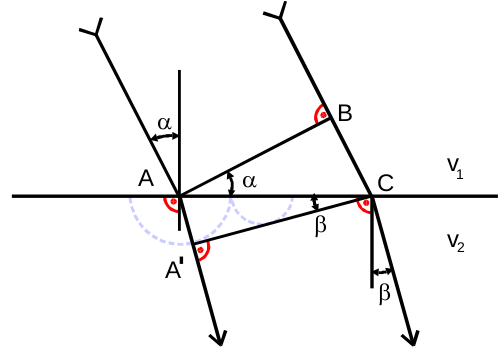
\includegraphics[height=5cm]{huygen.png}
  \caption{Brechung an einer Grenzfläche mit dem Huygenschen Prinzip.}
  \label{fig:huyg}
  \cite{skript}
\end{figure}

Die Elementarwellen an Punkt $A$ breiten sich mit einer anderen Geschwindigkeit
aus, als die Elementarwellen, die von Punkt $B$ ausgehen, da sie sich in
unterschiedlichen Medien bewegen. Wenn die Elementarwellen bzw. die
durch sie neu gebildete Wellenfront die Grenzfläche erreichen breiten sie sich
ebenfalls mit einer anderen Geschwindigkeit aus als zuvor. Durch Überlagerung
der Elementarwellen aus Punkt $A'$ und $C$ baut sich eine neue Wellenfront auf.
Dadurch ändert sich der Winkel zur Grenzebene gegenüber dem Einfallswinkel.

Aus Abbildung \ref{fig:huyg} kann das Snelliussche Brechungsgesetz hergeleitet werden,
dieses lautet:
\begin{equation}
  \frac{\sin{(\alpha)}}{\sin{(\beta)}}=\frac{v_1}{v_2}=n.
  \label{eqn:brechung}
\end{equation}

\subsection{Dispersionsgleichung}
Die Dispersionsgleichung beschreibt den Zusammenhang zwischen Wellenlänge
und Brechungsindex. Um sie herzuleiten darf das Medium nicht als Kontinuum
angesehen werden, sondern es muss die elektrische Ladungsverteilung durch
Elektronen und Ionenrümpfen berücksichtigt werden. Diese befinden sich in einer Gleichgewichtslage, welche
durch das elektrische Wechselfeld der Lichtwellen zu erzwungen Schwingungen
angeregt werden. Allgemein existiert bei Schwingungsphänomenen eine Resonanzfrequenz,
hier wird jedoch der Wellenlängenbereich betrachtet, in dem keine
Resonanz, also nur geringe Absorption auftritt. Für andere Wellenlängenbereiche
muss das Problem quantenmechanisch betrachtet werden.

Fällt Licht auf eine Materieschicht, so wirkt duch das elektrische Feld eine
periodische Kraft
\begin{equation}
  \vec{F_e}=q_h\cdot \vec{E}
\end{equation}
auf die Ladungen der Materieschicht. (Die magnetische Wechselwirkung durch
die Lorentzkraft kann vernachlässigt werden.)
Dadurch werden die Teilchen um $\vec{x_h}$ aus Ihrer Ruhelage ausgelenkt und es entsteht
ein elektrische Dipol.
Gleichzeitig wirkt auf die Teilchen eine rücktreibende Kraft
\begin{equation}
  \vec{F_{r,h}}=a_h \vec{x_h}
\end{equation}
und eine Reibungskraft
\begin{equation}
  \vec{F_{d,h}}=f_h \frac{\delta \vec{x_h}}{\delta t}.
\end{equation}

Daraus ergibt sich die Differentialgleichung
\begin{equation}
  m_h\frac{d^{2}\vec{x_h}}{dt^{2}}+f_h\frac{d\vec{x_h}}{dt}+a_h\vec{x_h}=q_h\vec{E_0}\exp{(t\omega t)},
\end{equation}
durch Umformungen mit der Relation $\sum_{h}{N_h q_h \vec{x_h}}$ und der
Maxwellrealtion $n^{2}=\epsilon$ ergibt sich
ein Ausdruck für den Brechungsindex:
\begin{equation}
  \tilde{n}^2=1+ \sum_{h} \frac{1}{\omega^{2}_h - \omega^{2}+i\frac{f_h}{m_h}\omega}
  \frac{N_q q^{2}_h}{m_h \epsilon_0}.
  \label{eqn:ntilde}
\end{equation}

Durch $\tilde{}$\;wird angedeutet, dass die Dielektrizitätskonstante und der
Brechungsindex als komplexe Größe angesetzt werden müssen. Es gilt:

\begin{equation}
  \tilde{n}= n(1-ik),
\end{equation}

dann ist der Realteil $n$ der nach Gleichung \ref{eqn:n} definierte Brechungsindex.
Der Imaginärteil ist relevant für die Absorption.

In Bereichen hoher Absorption trifft dieses Modell nur schlecht zu, daher
werden nur Bereiche geringer Absorption betrachtet, in diesen gilt:
\begin{equation}
  n^{2}k\approx 0.
\end{equation}
 Mit dieser Relation folgt aus Gleichung \ref{eqn:ntilde} eine Formel für den
 Brechungsindex:
 \begin{equation}
   n^{2}(\lambda)= 1+ \sum_{h}\frac{N_h q^{2}_h}{4\pi^{2}c^2 \epsilon_0 m_h}
   \frac{\lambda^2 \lambda^{2}_h}{\lambda^2 - \lambda^{2}_h}.
   \label{eqn:nquadrat}
 \end{equation}

Im Folgenden wird angenommen, dass die betrachtete Materie eine Absorptionsstelle
bei $\lambda_1$ besitzt. Die auf die Materie gestrahlte Wellenlänge $\lambda$
kann nun größer oder klein sein als die Absorptionswellenlänge, daher sind
folgende Fallunterscheidungen zu treffen.

\subsection{Fallunterscheidung für Wellenlängen größer als die Absorptionswellenlänge} %$\lambda >> \lambda_1$}
Wird die Gleichung \ref{eqn:nquadrat} in eine Potenzreihe entwickelt ergibt
sich:
\begin{equation}
  n^2(\lambda)=1+\frac{N_1 q^{2}_1 \lambda_{1}^{2}}{4\pi^2c^2\epsilon_0 m_1}
  \Bigr(1+\Bigr(\frac{\lambda_1}{\lambda}\Bigl)^2 +\Bigl(\frac{\lambda_1}{\lambda}\Bigr)^4+...).
  \label{eqn:nquadratpotenz1}
\end{equation}
Vereinfacht kann auch
\begin{equation}
 n^2(\lambda)= A_0+\frac{A_2}{\lambda^2}+\frac{A_4}{\lambda^4}+...
 \label{eqn:nquadrat1}
\end{equation}
geschrieben werden.
Dabei gilt für die Koeffizienten $A_0,A_2,A_4>0$.
Für diesen Fall nimmt die Dispersionskurve die Gestalt aus
Abbildung \ref{fig:krumminnen} an.

\begin{figure}[H]
  \centering
  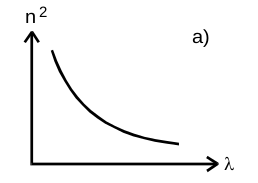
\includegraphics[height=3cm]{n1.png}
  \caption{Verlauf der Dispersionskurve.}
  \label{fig:krumminnen}
  \cite{skript}
\end{figure}

Aus einem Koeffizientenvergleich der Gleichungen \ref{eqn:nquadratpotenz1}
und \ref{nquadrat1} lässt sicf fhlgender Ausdruck für die
Absorptionsstelle $\lambda_1$ schreiben:
\begin{equation}
  \lambda_1=\sqrt{\frac{A_2}{A_0}-1}
  \label{eqn:absorption}
\end{equation}

\subsection{Fallunterscheidung für Wellenlängen kleiner als die Absorptionswellenlänge}% $\lambda=\lambda_1$}
Für diesen Fall nähert sich die verwendete Wellenlänge von einem kurzwelligeren
Bereich an die Absorptionsstelle an. Hier lässt sich Gleichung
\ref{eqn:nquadrat} zu
\begin{equation}
  n^2(\lambda)=1-\frac{N_1 q^{2}_1}{4\pi^2c^2\epsilon_0 m_1}
  \Bigr(\Bigr(\lambda^2+\frac{\lambda^4}{\lambda^{2}_1}+\frac{\lambda^6}{\lambda^{4}_1}...).
  \label{eqn:nquadratpotenz2}
\end{equation}
entwickeln. Mit den Koeffizienten $A'_i>0$ ergibt sich vereinfacht:
\begin{equation}
  n^2(\lambda)=1-A'_2 \lambda^2 -A'_4 \lambda^4-....
  \label{eqn:nquadrat2}
\end{equation}

Für diesen Fall ist die Dispersionskurve in Abbildung \ref{fig:krummaußen}
dargestellt.

\begin{figure}[H]
  \centering
  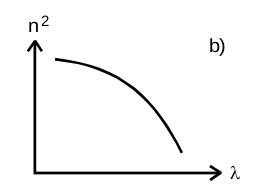
\includegraphics[height=3cm]{n2.png}
  \caption{Verlauf der Dispersionskurve.}
  \label{fig:krummaußen}
  \cite{skript}
\end{figure}


Beide Abbildungen \ref{fig:krumminnen} und \ref{fig:krummaußen} haben gemeinsam, dass
der Brechungsindex mit zunehmender Wellenlänge abnimmt. Dieses Verhalten wird als
normale Dispersion bezeichnet. Der umgekehrte Fall, also die Zunahme des
Brechungsindex mit der Wellenlänge wird anormale Dispersion genannt.
Anormale Dispersion kann nicht durch die Formeln \ref{eqn:nquadrat1} und
\ref{eqn:nquadrat2} beschrieben werden.

\subsection{Auflösungsvermögen eines Prismen-Spektralapparates}
Um die Frage zu beantworten, wie gering der Wellenlängenunterschied $\Delta \lambda$
werden darf, dass zwei benachbarte Spektrallinien noch getrennt werden können,
wird das Auflösungsvermögen $A$ definiert:
\begin{equation}
  A=\frac{\lambda}{\Delta \lambda}.
  \label{eqn:auflösung}
\end{equation}
Dabei bezeichnet $\lambda$ die gemittelte Wellenlänge der beiden
Spektrallinien.
Das Auflösungsvermögen ist durch Beugungserscheinungen beschränkt, denn
das Prisma wirkt aufgrund seiner endlichen Größe wie eine
spaltförmige Blende. Deshalb wird in der Brennebene kein scharfes Bild, sondern
eine Beugungsfigur abgebildet.
Fallen nun zwei Wellen mit leicht unterschiedlicher Wellenlänge in den
Spektralapparat, so werden sie aufgrund der Dispersion unterschiedlich
stark gebrochen.Der Richtungsunterschied sei $\Delta \eta$.
Es entstehen in der Brennebene als zwei leicht unterschiedliche Brechungsfiguren,
deren Maximum leicht gegeneinander verschoben ist.Siehe dazu Abbildung
\ref{fig:auflösung}.

\begin{figure}[H]
  \centering
  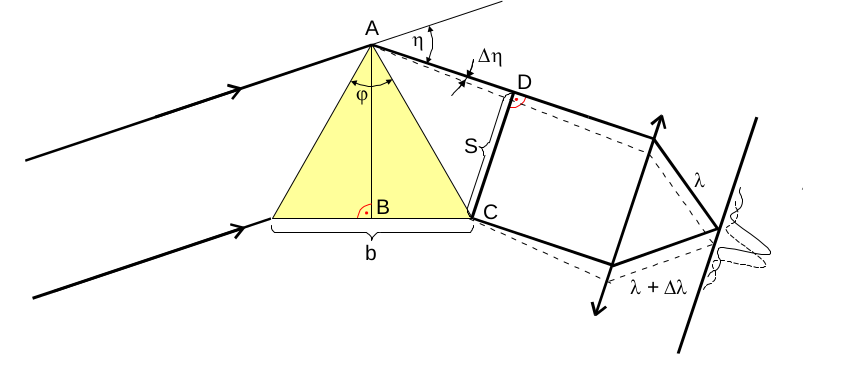
\includegraphics[width=11cm]{beug.png}
  \caption{Skizze eines Prismen-Spektralapparates.}
  \label{fig:auflösung}
  \cite{skript}
\end{figure}

Eine Trennung der Spektrallinien soll noch möglich sein, wenn ein Maximum
genau in ein Minimum der anderen Wellenlänge fällt.
Das erste Beugungsminimum liegt immer an der Stelle
\begin{equation}
  \sin{\theta_{min}}=\frac{\lambda}{s}.
\end{equation}
(s=Spaltbreite)
Für den Richtungsunterschied $\Delta\eta$ folgt
\begin{equation}
  \sin({\Delta\eta})=\frac{\lambda}{s}
  \label{eqn:sineta}
\end{equation}
mit der Kleinwinkelnäherung ergibt sich:
\begin{equation}
  \Delta \eta =\frac{\lambda}{s}.
  \label{eqn:deltaeta}
\end{equation}

Nach weiteren Umformungen und der Verwendung der Basisbreite $b$ des
Prismas lässt sich folgender Ausdruck für das Auflösungsvermögen
herleiten:
\begin{equation}
  \frac{\lambda}{\Delta \lambda}=b\frac{dn}{d\lambda}.
  \label{eqn:auflösungsvermögen}
\end{equation}

Die Ableitung von $n(\lambda)$ nach $\lambda$ ergibt sich zu
\begin{equation}
  \frac{dn(\lambda)}{d\lambda}=\frac{d}{d\lambda}\sqrt{A_0+\frac{A_2}{\lambda^2}}
  =-\frac{A_2}{\lambda^3}\sqrt{A_0+\frac{A_2}{\lambda^2}},
\end{equation}
somit kann das Auflösungsvermögen über
\begin{equation}
  A=b\frac{A_2}{\lambda^3}{\sqrt{A_0+\frac{A_2}{\lambda^2}}}.
  \label{eqn:auflösungsver}
\end{equation}
berechent werden.

\subsection{Theoretischer Anhang}
Um eine möglichst genaue Dispersionsgleichung zu erhalten, muss
entschieden werden, welche der möglichen Dispersionsgleichungen
\ref{eqn:nquadrat1} und \ref{eqn:nquadrat2} sich den Wertepaaren
am besten anpasst. Um das herauszufinden kann die Methode der
kleinsten Quadrate verwendet werden um die optimalen Koeffizienten
$A_i$ und $A'_1$ zu bestimmen.
Die Summe der Abweichungsquadrate errechnet sich nach:
\begin{align}
  s_{n}^{2}&=\frac{1}{z-2}\sum_{i=1}^{z} \Bigl(n^2(\lambda_i)-A_0-\frac{a_2}{\lambda_{i}^{2}}\Bigr) \\
  \text{bzw.}\\
  s_{n}'^{2}&=\frac{1}{z-2}\sum_{i=1}^{z} \Bigl(n^2(\lambda_i)-A'_0+A'_{2}\lambda_{i}^{2}\Bigr) \\.
  \label{eqn:abweichungquadrat}
\end{align}
Es wird die Dispersionsrelation mit dem kleineren $s^2$ als passend angenommen.

Nicht jedes Material streut die Farben gleich stark, daher wird mit
\begin{equation}
  \nu=\frac{n_D -1}{n_F-n_C}
  \label{eqn:abbel}
\end{equation}
die Abbelsche Zahl definiert, die ein Maß für die Farbstreuung darstelt.
Dabei sind $n_C, n_D und n_F$ als die Brechungsindices der Frauenhoferschen
Linien definiert.
$\lambda_C=656\;nm,\;\lambda_D=589\;nm,\;\lambda_F=486\;nm$
